\scanpage{22}
% Reader A independent proposed transcription. Manual geometry; source-only validation.
% Drawing coordinate system: original full scan, origin upper left; x right, y down.
% TikZ units x=0.085 mm, y=-0.085 mm; all inner scopes use the same units.
% Every visible label occurs once. Phantom copies retain editorial state without extra ink.
\figure{\begin{tikzpicture}[x=0.085mm,y=-0.085mm,baseline=0pt,
  every node/.style={anchor=base west,inner sep=0pt,outer sep=0pt}]
\path[use as bounding box] (240,60) rectangle (1681,2095);
% LABEL T01: owns exactly the visible contents of this node; state=deleted.
\node at (294,126) {\resizebox{7.735mm}{!}{\rlap{\unsure{Un|On}}\phantom{\deleted{\unsure{Un|On}}}}};
% LABEL T02: owns exactly the visible contents of this node; state=deleted.
\node at (417,139) {\resizebox{20.400mm}{!}{\rlap{\unsure{procède|procéde|procédé|procede}}\phantom{\deleted{\unsure{procède|procéde|procédé|procede}}}}};
% LABEL T03: owns exactly the visible contents of this node; state=deleted.
\node at (680,145) {\resizebox{54.060mm}{!}{\rlap{par récurrence sur}\phantom{\deleted{par récurrence sur}}}};
% LABEL T04: owns exactly the visible contents of this node; state=deleted.
\node at (1360,154) {\resizebox{18.275mm}{!}{\rlap{$\operatorname{card} K$,}\phantom{\deleted{$\operatorname{card} K$,}}}};
% LABEL T05: owns exactly the visible contents of this node; state=inserted.
\node at (315,177) {\resizebox{42.585mm}{!}{\rlap{On note d'abord que}\phantom{\inserted{On note d'abord que}}}};
% LABEL T06: owns exactly the visible contents of this node; state=deleted.
\node at (256,227) {\resizebox{47.855mm}{!}{\rlap{pour prouver que}\phantom{\deleted{pour prouver que}}}};
% BEGIN A022-G01-opening-cancellations
% Observed locus [284, 96, 1581, 230]; complete ownership: two actual cancellation runs; the six opening text labels remain outside
\draw[line width=.45pt] (335,108) .. controls (690,103) and (1060,104) .. (1390,114) .. controls (1490,119) and (1541,124) .. (1569,126);
\draw[line width=.45pt] (284,224) .. controls (434,214) and (642,218) .. (817,213);
% END A022-G01-opening-cancellations% BEGIN B022-M01; observed full-scan box [313, 224, 334, 239].
% Ownership: Short detached slash below pour; the word pour stays in T03.
% Role/state: Shape supported; attachment, role, hand and surface origin remain unresolved.
% Complete reading/state candidates: visible short slash; no character assigned
\node[anchor=base west,inner sep=0pt,outer sep=0pt] at (313,239) {\unsure{%
\begin{tikzpicture}[x=0.085mm,y=-0.085mm,baseline=(B),every node/.style={inner sep=0pt,outer sep=0pt,anchor=base west}]
\path[use as bounding box] (0,0) rectangle (21,15);
\coordinate (B) at (0,15);
\begin{scope}[shift={(-313,-224)}]
\draw[line width=.4pt,line cap=round] (318,234) -- (331,228);
\end{scope}
\end{tikzpicture}%
}};
% END B022-M01

% LABEL T07: owns exactly the visible contents of this node; state=live.
\node at (883,222) {\resizebox{7.395mm}{!}{(si}};
% LABEL T08: owns exactly the visible contents of this node; state=live.
\node at (1014,218) {\resizebox{9.435mm}{!}{$V=X$}};
% BEGIN A022-G02-initial-separator
% Observed locus [1124, 190, 1137, 222]; complete ownership: the one short upright separator after X; no adjacent word or letter
% Complete candidate/state annotation: \setminus primary; literal nearly upright run retained without changing its direction
\draw[line width=.7pt] (1128,196) .. controls (1130,203) and (1129,213) .. (1130,219);
% END A022-G02-initial-separator
% BEGIN B022-G02; observed full-scan box [1153, 166, 1218, 253].
% Ownership: Top union operator and its alpha-in-K lower limit.
% Role/state: The upper-left stem is interrupted before the returning bowl; both runs are preserved.
\draw[line width=.45pt,line cap=round] (1168,175) .. controls (1169,185) and (1170,190) .. (1170,196);
\draw[line width=.45pt,line cap=round] (1171,202) .. controls (1173,216) and (1193,218) .. (1205,204) .. controls (1216,189) and (1209,179) .. (1200,169);
\node[font=\scriptsize,anchor=base west,inner sep=0pt,outer sep=0pt] at (1157,244) {$\alpha\in K$};
% END B022-G02

% BEGIN A022-S01
% Observed locus [1211, 151, 1290, 224]; complete ownership: complete Sigma body, head, hat, raised sign and index; no adjacent relation or word
% Complete candidate/state annotation: \widehat{\Sigma}_{\alpha}^{+}; short head role: head/retrace or separate upper run, no extra mathematical operation selected
\node[anchor=base west,inner sep=0pt,outer sep=0pt] at (1211,151) {\unsure{%
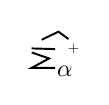
\begin{tikzpicture}[x=0.085mm,y=-0.085mm,baseline=0pt, every node/.style={anchor=base west,inner sep=0pt,outer sep=0pt}]
\path[use as bounding box] (0,0) rectangle (79,73);
\begin{scope}[shift={(-1211,-151)}]
\draw[line width=.7pt] (1217,182) -- (1252,183);
\draw[line width=.7pt] (1217,188) -- (1243,197) -- (1217,211) -- (1252,211);
\draw[line width=.7pt] (1232,169) -- (1257,157) -- (1272,168);
\node at (1271,188) {\resizebox{1.445mm}{!}{$+$}};
\node at (1255,224) {\resizebox{1.955mm}{!}{$\alpha$}};
\end{scope}
\end{tikzpicture}%
}};
% END A022-S01
% LABEL T09: owns exactly the visible contents of this node; state=live.
\node at (1305,229) {\resizebox{1.530mm}{!}{,}};
% LABEL T10: owns exactly the visible contents of this node; state=live.
\node at (1338,220) {\resizebox{5.185mm}{!}{les}};
% BEGIN A022-S02
% Observed locus [1445, 159, 1520, 226]; complete ownership: complete Sigma body, head, hat, raised sign and index; no adjacent relation or word
% Complete candidate/state annotation: \widehat{\Sigma}_{\alpha}^{+}
\draw[line width=.7pt] (1452,184) -- (1493,186);
\draw[line width=.7pt] (1453,191) -- (1478,198) -- (1451,211) -- (1497,212);
\draw[line width=.7pt] (1467,174) -- (1483,164) -- (1497,173);
\node at (1504,190) {\resizebox{1.445mm}{!}{$+$}};
\node at (1494,225) {\resizebox{1.955mm}{!}{$\alpha$}};
% END A022-S02
% BEGIN B022-G03; observed full-scan box [1526, 182, 1635, 231].
% Ownership: Opening curve and immediately adjoining alpha-in-K; no second printed alpha is outside this group.
% Role/state: Root §02 resolves the opening curve as a parenthesis; its adjoining alpha-in-K remains owned here.
% Root selected reading: (\alpha\in K
\node[anchor=base west,inner sep=0pt,outer sep=0pt] at (1526,231) {%
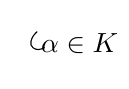
\begin{tikzpicture}[x=0.085mm,y=-0.085mm,baseline=(B),every node/.style={inner sep=0pt,outer sep=0pt,anchor=base west}]
\path[use as bounding box] (0,0) rectangle (109,49);
\coordinate (B) at (0,49);
\begin{scope}[shift={(-1526,-182)}]
\draw[line width=.4pt,line cap=round] (1540,188) .. controls (1530,197) and (1528,208) .. (1534,212) .. controls (1539,216) and (1545,215) .. (1551,212);
\node[font=\normalsize,anchor=base west,inner sep=0pt,outer sep=0pt] at (1546,219) {$\alpha\in K$};
\node[font=\scriptsize,anchor=base west,inner sep=0pt,outer sep=0pt] at (1526,231) {\phantom{$(\alpha\in K$}};
\end{scope}
\end{tikzpicture}%
};
% END B022-G03
% BEGIN B022-G04; observed full-scan box [1639, 208, 1678, 301].
% Ownership: Both surviving right-edge closure runs, after the alpha-in-K line and after disjoints.
% Role/state: One spanning close versus two distinct closes is unresolved; the physical edge supplies no connecting ink.
% Root complete reading/state candidates: one spanning ) | two separate ) )
\node[anchor=base west,inner sep=0pt,outer sep=0pt] at (1639,301) {\unsure{%
\begin{tikzpicture}[x=0.085mm,y=-0.085mm,baseline=(B),every node/.style={inner sep=0pt,outer sep=0pt,anchor=base west}]
\path[use as bounding box] (0,0) rectangle (39,93);
\coordinate (B) at (0,93);
\begin{scope}[shift={(-1639,-208)}]
\draw[line width=.3pt,line cap=round] (1662,213) .. controls (1669,219) and (1672,229) .. (1676,240);
\draw[line width=.4pt,line cap=round] (1666,262) .. controls (1662,276) and (1653,287) .. (1644,296);
\node[font=\scriptsize,anchor=base west,inner sep=0pt,outer sep=0pt] at (1639,301) {\phantom{\unsure{one spanning )|two separate ) )}}};
\end{scope}
\end{tikzpicture}%
}};
% END B022-G04

% LABEL T11: owns exactly the visible contents of this node; state=live.
\node at (1452,270) {\resizebox{17.340mm}{!}{etant disjoints}};
% BEGIN B022-G05; observed full-scan box [1077, 250, 1270, 306].
% Ownership: Complete hooked lower bracket and the descending equality strokes; no central brace cusp is supplied.
% Role/state: The bracket attaches the next intersection to X setminus the union.
\draw[line width=.45pt,line cap=round] (1083,255) .. controls (1078,264) and (1079,272) .. (1087,273) .. controls (1137,272) and (1205,276) .. (1251,273) .. controls (1266,273) and (1267,262) .. (1260,261);
\draw[line width=.5pt,line cap=round] (1161,284) -- (1162,299);
\draw[line width=.5pt,line cap=round] (1171,284) -- (1172,301);
% END B022-G05

% BEGIN B022-G06; observed full-scan box [1102, 306, 1166, 385].
% Ownership: Inserted intersection sign and its alpha-in-K lower limit.
% Role/state: Added below the bracket; its formula continues with S03.
\draw[line width=.55pt,line cap=round] (1126,338) .. controls (1120,321) and (1130,312) .. (1141,313) .. controls (1154,311) and (1164,320) .. (1164,337);
\node[font=\scriptsize,anchor=base west,inner sep=0pt,outer sep=0pt] at (1106,379) {$\alpha\in K$};
\node[font=\scriptsize,anchor=base west,inner sep=0pt,outer sep=0pt] at (1102,385) {\phantom{$\inserted{\bigcap_{\alpha\in K}}$}};
% END B022-G06

% BEGIN B022-S03; observed full-scan box [1164, 306, 1245, 356].
% Ownership: Complete Sigma glyph, its head/body, index \alpha and raised -; no adjoining word.
% Role/state: The head and body form the locally observed connected letter shape.
% Complete reading/state candidates: \Sigma_{\alpha}^{-}
\draw[line width=.45pt,line cap=round,line join=round] (1200,314) -- (1172,313) .. controls (1165,315) and (1166,320) .. (1175,321) -- (1195,326) -- (1172,340) -- (1203,341);
\node[font=\scriptsize,anchor=base west,inner sep=0pt,outer sep=0pt] at (1205,352) {$\alpha$};
\node[font=\scriptsize,anchor=base west,inner sep=0pt,outer sep=0pt] at (1213,322) {$-$};
\node[font=\scriptsize,anchor=base west,inner sep=0pt,outer sep=0pt] at (1164,356) {\phantom{$\Sigma_{\alpha}^{-}$}};
% END B022-S03

% BEGIN A022-G07-first-brace-arrow
% Observed locus [413, 286, 584, 482]; complete ownership: main left brace with closed middle loop, marginal arrow shaft and two-leg head; trivial text is outside
\draw[line width=.6pt] (549,294) .. controls (555,321) and (550,368) .. (546,380) .. controls (542,396) and (533,390) .. (540,383) .. controls (555,378) and (558,432) .. (554,456) .. controls (554,469) and (557,477) .. (560,479);
\draw[line width=.45pt] (457,445) .. controls (510,443) and (548,439) .. (581,435);
\draw[line width=.65pt] (575,431) -- (582,435) -- (574,438);
% END A022-G07-first-brace-arrow
% LABEL T12: owns exactly the visible contents of this node; state=live.
\node at (413,449) {\resizebox{9.265mm}{!}{trivial}};
% LABEL T13: owns exactly the visible contents of this node; state=live.
\node at (582,343) {\resizebox{28.815mm}{!}{$\overline V\cap E_\alpha\ne\varnothing$}};
% LABEL T14: owns exactly the visible contents of this node; state=live.
\node at (592,460) {\resizebox{6.545mm}{!}{$V\cap$}};
% BEGIN A022-S04
% Observed locus [678, 400, 780, 463]; complete ownership: complete Sigma body, head, raised sign and index; no adjacent relation or word
% Complete candidate/state annotation: \Sigma_{\alpha}^{-}
\draw[line width=.7pt] (686,411) -- (728,405);
\draw[line width=.7pt] (685,419) -- (715,427) -- (687,446) -- (730,445);
\node at (746,411) {\resizebox{1.445mm}{!}{$-$}};
\node at (738,462) {\resizebox{1.955mm}{!}{$\alpha$}};
% END A022-S04
% BEGIN B022-G08; observed full-scan box [794, 384, 925, 485].
% Ownership: The old relation and its old empty-set glyph, including their local cancellation strokes; replacement is T10.
% Role/state: C022-R03 retained. The short upright can belong to the relation or to its cancellation; all old ink is retained.
% Complete reading/state candidates: \deleted{\ne\varnothing} | \deleted{=\varnothing}
\node[anchor=base west,inner sep=0pt,outer sep=0pt] at (794,485) {\unsure{%
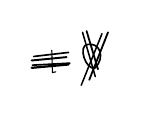
\begin{tikzpicture}[x=0.085mm,y=-0.085mm,baseline=(B),every node/.style={inner sep=0pt,outer sep=0pt,anchor=base west}]
\path[use as bounding box] (0,0) rectangle (131,101);
\coordinate (B) at (0,101);
\begin{scope}[shift={(-794,-384)}]
\draw[line width=.6pt,line cap=round] (803,427) -- (855,421);
\draw[line width=.6pt,line cap=round] (801,440) -- (857,437);
\draw[line width=.4pt,line cap=round] (830,418) -- (831,451) -- (836,450);
\draw[line width=.7pt,line cap=round] (800,433) -- (852,428);
\draw[line width=.8pt,line cap=round] (800,444) -- (855,439);
\draw[line width=.6pt,line cap=round] (884,409) .. controls (868,410) and (881,449) .. (895,444) .. controls (910,428) and (902,406) .. (884,409);
\draw[line width=.55pt,line cap=round] (905,393) -- (874,470);
\draw[line width=.55pt,line cap=round] (876,391) -- (895,457);
\draw[line width=.65pt,line cap=round] (882,389) -- (899,446);
\draw[line width=.65pt,line cap=round] (914,391) -- (886,462);
\node[font=\scriptsize,anchor=base west,inner sep=0pt,outer sep=0pt] at (794,485) {\phantom{$\deleted{\unsure{\ne|=}\varnothing}$}};
\end{scope}
\end{tikzpicture}%
}};
% END B022-G08

% LABEL T15: owns exactly the visible contents of this node; state=live.
\node at (938,449) {\resizebox{6.715mm}{!}{$\ne\varnothing$}};
% LABEL T16: owns exactly the visible contents of this node; state=live.
\node at (1095,441) {\resizebox{17.000mm}{!}{alors que}};
% LABEL T17: owns exactly the visible contents of this node; state=live.
\node at (1340,445) {\resizebox{5.185mm}{!}{$V\cap$}};
% BEGIN A022-S05
% Observed locus [1408, 390, 1486, 449]; complete ownership: complete Sigma body, head, raised sign and index; no adjacent relation or word
% Complete candidate/state annotation: \Sigma_{\alpha}^{+}
\draw[line width=.7pt] (1415,402) -- (1444,402);
\draw[line width=.7pt] (1416,407) -- (1436,414) -- (1416,432) -- (1446,432);
\node at (1464,404) {\resizebox{1.445mm}{!}{$+$}};
\node at (1447,444) {\resizebox{1.955mm}{!}{$\alpha$}};
% END A022-S05
% LABEL T18: owns exactly the visible contents of this node; state=live.
\node at (1498,447) {\resizebox{7.735mm}{!}{$=\varnothing$}};
% LABEL T19: owns exactly the visible contents of this node; state=live.
\node at (258,594) {\resizebox{70.125mm}{!}{De façon précise, je dis que}};
% BEGIN A022-M01-precise-upper-tick
% Observed locus [630, 563, 638, 571]; complete ownership: one short upper tick near précise; the word and its acute remain in T19
\node[anchor=base west,inner sep=0pt,outer sep=0pt] at (630,563) {\unsure{%
\begin{tikzpicture}[x=0.085mm,y=-0.085mm,baseline=0pt, every node/.style={anchor=base west,inner sep=0pt,outer sep=0pt}]
\path[use as bounding box] (0,0) rectangle (8,8);
\begin{scope}[shift={(-630,-563)}]
\draw[line width=.75pt] (633,565) -- (634,568);
\end{scope}
\end{tikzpicture}%
}};
% END A022-M01-precise-upper-tick
% LABEL T20: owns exactly the visible contents of this node; state=live.
\node at (606,729) {\resizebox{23.715mm}{!}{$\overline V\cap E_\alpha=$}};
% BEGIN A022-S06
% Observed locus [906, 642, 1019, 732]; complete ownership: complete Sigma body, head, closure rule, raised sign and index; no adjacent relation or word
% Complete candidate/state annotation: \overline{\Sigma}_{\alpha}^{-}
\draw[line width=.7pt] (915,668) -- (965,668);
\draw[line width=.7pt] (915,668) -- (941,690) -- (913,717) -- (964,713);
\draw[line width=.7pt] (922,652) -- (993,649);
\node at (987,679) {\resizebox{1.445mm}{!}{$-$}};
\node at (967,729) {\resizebox{1.955mm}{!}{$\alpha$}};
% END A022-S06
% LABEL T21: owns exactly the visible contents of this node; state=live.
\node at (1038,722) {\resizebox{11.730mm}{!}{$\cap E_\alpha$}};
% LABEL T22: owns exactly the visible contents of this node; state=live.
\node at (1249,712) {\resizebox{34.680mm}{!}{(qui est donc $\ne\varnothing$)}};
% BEGIN A022-G10-lower-annotations
% State alternatives: live inserted pair | deleted inserted pair; the frame top belongs once to G14.
\node[anchor=base west,inner sep=0pt,outer sep=0pt] at (680,733) {\unsure{%
\begin{tikzpicture}[x=0.085mm,y=-0.085mm,baseline=0pt,every node/.style={anchor=base west,inner sep=0pt,outer sep=0pt}]
\path[use as bounding box] (0,0) rectangle (529,80);
\begin{scope}[shift={(-680,-733)}]
\draw[line width=.6pt] (688,751) -- (696,766);
\draw[line width=.6pt] (699,752) -- (706,771);
\node at (725,802) {\resizebox{6.205mm}{!}{$\overline V\cap$}};
% BEGIN A022-S07
% Observed locus [800, 739, 876, 805]; complete ownership: complete Sigma body, head, hat, raised sign and index; no adjacent relation or word
% Complete candidate/state annotation: \widehat{\Sigma}_{\alpha}^{+}
\draw[line width=.7pt] (809,767) -- (844,764);
\draw[line width=.7pt] (810,773) -- (837,779) -- (807,790) -- (848,790);
\draw[line width=.7pt] (815,754) -- (835,744) -- (849,751);
\node at (850,771) {\resizebox{1.445mm}{!}{$+$}};
\node at (847,801) {\resizebox{1.955mm}{!}{$\alpha$}};
% END A022-S07
% BEGIN A022-G11-right-connector
% Observed locus [1010, 734, 1074, 756]; complete ownership: three short oblique traces touching the closure rule owned by S08; no second horizontal rule
% Complete candidate/state annotation: \unsure{\deleted{=}|=|\Rightarrow}
\node[anchor=base west,inner sep=0pt,outer sep=0pt] at (1010,734) {\unsure{%
\begin{tikzpicture}[x=0.085mm,y=-0.085mm,baseline=0pt, every node/.style={anchor=base west,inner sep=0pt,outer sep=0pt}]
\path[use as bounding box] (0,0) rectangle (64,22);
\begin{scope}[shift={(-1010,-734)}]
\draw[line width=.65pt] (1015,751) -- (1028,742);
\draw[line width=.65pt] (1046,740) -- (1055,749);
\draw[line width=.65pt] (1063,739) -- (1070,750);
\node[overlay] at (1010,750) {\phantom{$\unsure{\deleted{=}|=|\Rightarrow}$}};
\end{scope}
\end{tikzpicture}%
}};
% END A022-G11-right-connector
% BEGIN A022-S08
% Observed locus [1003, 739, 1091, 797]; complete ownership: complete Sigma body, head, closure rule, raised sign and index; no adjacent relation or word
% Complete candidate/state annotation: \overline{\Sigma}_{\alpha}^{-}
\draw[line width=.7pt] (1009,764) -- (1038,762);
\draw[line width=.7pt] (1008,769) -- (1033,775) -- (1008,785) -- (1040,785);
\draw[line width=.7pt] (1011,750) -- (1069,749);
\node at (1053,767) {\resizebox{1.445mm}{!}{$-$}};
\node at (1046,794) {\resizebox{1.955mm}{!}{$\alpha$}};
% END A022-S08
\node at (1091,789) {\resizebox{2.295mm}{!}{$\cap$}};
% BEGIN A022-S09
% Observed locus [1122, 727, 1186, 790]; complete ownership: complete Sigma body, head, hat, raised sign and index; no adjacent relation or word
% Complete candidate/state annotation: \widehat{\Sigma}_{\alpha}^{+}
\draw[line width=.7pt] (1128,752) -- (1155,750);
\draw[line width=.7pt] (1128,752) -- (1150,759) -- (1127,772) -- (1159,772);
\draw[line width=.7pt] (1130,741) -- (1149,731) -- (1163,738);
\node at (1165,757) {\resizebox{1.445mm}{!}{$+$}};
\node at (1160,786) {\resizebox{1.955mm}{!}{$\alpha$}};
% END A022-S09
\node[overlay] at (716,804) {\phantom{$\inserted{\overline V\cap\widehat\Sigma_\alpha^+}$}};
\node[overlay] at (1006,796) {\phantom{$\inserted{\overline{\Sigma_\alpha^-}\cap\widehat\Sigma_\alpha^+}$}};
\end{scope}
\end{tikzpicture}%
}};
% END A022-G10-lower-annotations
% LABEL T23: owns exactly the visible contents of this node; state=deleted.
\node at (264,850) {\resizebox{17.425mm}{!}{\rlap{Comme}\phantom{\deleted{Comme}}}};
% LABEL T24: owns exactly the visible contents of this node; state=deleted.
\node at (615,849) {\resizebox{9.520mm}{!}{\rlap{$V\subset$}\phantom{\deleted{$V\subset$}}}};
% Root import C022-S10: original parent origin (245,630), original parent node anchor (495,214).
% Copied declared full base-west anchor (740,844), inner box xmin=-1, inner origin (741,844).
% Root §06 locally qualifies the physical head/return role; Sigma_alpha^- remains primary.
\node[anchor=base west,inner sep=0,outer sep=0,font=\small] at (740,844) {% BEGIN C022-S10
% full-scan origin/baseline (741, 844); local x=X-741, y=Y-844; x=0.085mm, y=-0.085mm.
% Owns one Sigma body, its short head, index \alpha, raised -, and the listed roof/bar/point only.
% Upper-run role: upper head lies immediately below the crossing frame; exact joining is crowded.
\unsure{\mbox{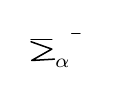
\begin{tikzpicture}[baseline={(0,0)},x=0.085mm,y=-0.085mm,line cap=round,line join=round]
\path[use as bounding box] (-1,-50) rectangle (86,12);
\draw[line width=.55pt] (4,-32) -- (35,-32);
\draw[line width=.55pt] (4,-29) -- (35,-18) -- (5,-1) -- (39,-3);
\node[anchor=base west,inner sep=0,outer sep=0,font=\scriptsize] at (40,9) {$\alpha$};
\draw[line width=.55pt] (65,-41) -- (77,-41);
\node[overlay,anchor=base west,inner sep=0,outer sep=0] at (0,0) {$\phantom{\deleted{\Sigma_{\alpha}^{-}}}$};
\end{tikzpicture}}}
% END C022-S10
};

% LABEL T25: owns exactly the visible contents of this node; state=deleted.
\node at (880,863) {\resizebox{1.530mm}{!}{\rlap{,}\phantom{\deleted{,}}}};
% LABEL T26: owns exactly the visible contents of this node; state=deleted.
\node at (922,847) {\resizebox{10.795mm}{!}{\rlap{on a}\phantom{\deleted{on a}}}};
% LABEL T27: owns exactly the visible contents of this node; state=deleted.
\node at (1161,845) {\resizebox{17.680mm}{!}{\rlap{$V\cap E_\alpha\subset$}\phantom{\deleted{$V\cap E_\alpha\subset$}}}};
% BEGIN R022-M01-plain-V-adjacent-point
% Root §07 supplies bbox (1158,843,1166,851), center (1162,847), radius .7.
% The base-west anchor and picture baseline copy bbox-left x=1158 and center y=847.
% Owns this locally qualified point alone; the adjoining plain V remains in A label T27.
\node[anchor=base west,inner sep=0pt,outer sep=0pt] at (1158,847) {\unsure{%
\begin{tikzpicture}[x=0.085mm,y=-0.085mm,baseline={(1158,847)}]
\path[use as bounding box] (1158,843) rectangle (1166,851);
\fill (1162,847) circle[radius=.7];
\end{tikzpicture}%
}};
% END R022-M01-plain-V-adjacent-point
% BEGIN A022-S11
% Observed locus [1398, 767, 1507, 851]; complete ownership: complete Sigma body, head, raised sign and index; no adjacent relation or word
% Complete candidate/state annotation: \overline{\Sigma_\alpha^-}|\Sigma_\alpha^-; upper-rule attachment unresolved; cancelled passage state retained
\node[anchor=base west,inner sep=0pt,outer sep=0pt] at (1398,767) {\unsure{%
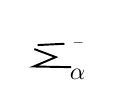
\begin{tikzpicture}[x=0.085mm,y=-0.085mm,baseline=0pt, every node/.style={anchor=base west,inner sep=0pt,outer sep=0pt}]
\path[use as bounding box] (0,0) rectangle (109,84);
\begin{scope}[shift={(-1398,-767)}]
\draw[line width=.7pt] (1413,793) -- (1453,791);
\draw[line width=.7pt] (1408,799) -- (1440,811) -- (1407,825) -- (1463,826);
% Upper rule is owned once by A022-G14-cancellation-frame, at x=1409..1494, y=773; do not draw it again here.
\node at (1465,795) {\resizebox{1.445mm}{!}{$-$}};
\node at (1461,845) {\resizebox{1.955mm}{!}{$\alpha$}};
\node[overlay] at (1398,851) {\phantom{$\deleted{\overline{\Sigma}_{\alpha}^{-}}$}};
\end{scope}
\end{tikzpicture}%
}};
% END A022-S11
% LABEL T28: owns exactly the visible contents of this node; state=deleted.
\node at (1510,849) {\resizebox{12.070mm}{!}{\rlap{$\cap E_\alpha$,}\phantom{\deleted{$\cap E_\alpha$,}}}};
% LABEL T29: owns exactly the visible contents of this node; state=deleted.
\node at (265,977) {\resizebox{17.680mm}{!}{\rlap{prouvons}\phantom{\deleted{prouvons}}}};
% LABEL T30: owns exactly the visible contents of this node; state=deleted.
\node at (582,958) {\resizebox{44.795mm}{!}{\rlap{l'inclusion inverse}\phantom{\deleted{l'inclusion inverse}}}};
% BEGIN A022-M02-left-upright
% Observed locus [246, 886, 257, 905]; complete ownership: one detached thin upright to left of the cancellation frame; no text
\node[anchor=base west,inner sep=0pt,outer sep=0pt] at (246,886) {\unsure{%
\begin{tikzpicture}[x=0.085mm,y=-0.085mm,baseline=0pt, every node/.style={anchor=base west,inner sep=0pt,outer sep=0pt}]
\path[use as bounding box] (0,0) rectangle (11,19);
\begin{scope}[shift={(-246,-886)}]
\draw[line width=.35pt] (253,890) .. controls (251,895) and (251,898) .. (251,903);
\end{scope}
\end{tikzpicture}%
}};
% END A022-M02-left-upright
% BEGIN B022-S12; observed full-scan box [557, 1019, 676, 1098].
% Ownership: Complete Sigma glyph, its head/body, outer bar, index \alpha and raised -; no adjoining word.
% Role/state: The head and body form the locally observed connected letter shape.
% Complete reading/state candidates: \overline{\Sigma_{\alpha}^{-}}
\draw[line width=.45pt,line cap=round,line join=round] (621,1047) -- (567,1051) .. controls (565,1055) and (594,1055) .. (610,1062) -- (570,1086) -- (635,1075);
\draw[line width=.45pt,line cap=round] (574,1031) .. controls (603,1031) and (631,1027) .. (665,1026);
\node[font=\scriptsize,anchor=base west,inner sep=0pt,outer sep=0pt] at (621,1092) {$\alpha$};
\node[font=\scriptsize,anchor=base west,inner sep=0pt,outer sep=0pt] at (648,1057) {$-$};
\node[font=\scriptsize,anchor=base west,inner sep=0pt,outer sep=0pt] at (557,1098) {\phantom{$\deleted{\overline{\Sigma_{\alpha}^{-}}}$}};
% END B022-S12

% LABEL T31: owns exactly the visible contents of this node; state=deleted.
\node at (681,1089) {\resizebox{35.190mm}{!}{\rlap{$\cap E_\alpha\subset\overline V\cap E_\alpha$}\phantom{\deleted{$\cap E_\alpha\subset\overline V\cap E_\alpha$}}}};
% LABEL T32: owns exactly the visible contents of this node; state=deleted.
\node at (281,1208) {\resizebox{7.735mm}{!}{\rlap{Soit}\phantom{\deleted{Soit}}}};
% LABEL T33: owns exactly the visible contents of this node; state=deleted.
\node at (482,1200) {\resizebox{5.525mm}{!}{\rlap{$x\in$}\phantom{\deleted{$x\in$}}}};
% BEGIN A022-S13
% Observed locus [589, 1136, 678, 1211]; complete ownership: complete Sigma body, head, closure rule, raised sign and index; no adjacent relation or word
% Complete candidate/state annotation: \overline{\Sigma}_{\alpha}^{-}
\draw[line width=.7pt] (598,1163) -- (636,1161);
\draw[line width=.7pt] (598,1168) -- (626,1178) -- (594,1195) -- (641,1194);
\draw[line width=.7pt] (601,1146) -- (668,1142);
\node at (650,1164) {\resizebox{1.445mm}{!}{$-$}};
\node at (641,1208) {\resizebox{1.955mm}{!}{$\alpha$}};
\node[overlay] at (589,1211) {\phantom{$\deleted{\overline{\Sigma}_{\alpha}^{-}}$}};
% END A022-S13
% LABEL T34: owns exactly the visible contents of this node; state=deleted.
\node at (681,1207) {\resizebox{10.625mm}{!}{\rlap{$\cap E_\alpha$,}\phantom{\deleted{$\cap E_\alpha$,}}}};
% LABEL T35: owns exactly the visible contents of this node; state=deleted.
\node at (862,1197) {\resizebox{18.615mm}{!}{\rlap{prouvons}\phantom{\deleted{prouvons}}}};
% LABEL T36: owns exactly the visible contents of this node; state=deleted.
\node at (1160,1198) {\resizebox{22.015mm}{!}{\rlap{$x\in\overline V\cap E_\alpha$}\phantom{\deleted{$x\in\overline V\cap E_\alpha$}}}};
% LABEL T37: owns exactly the visible contents of this node; state=deleted.
\node at (1461,1191) {\resizebox{5.355mm}{!}{\rlap{i.e.}\phantom{\deleted{i.e.}}}};
% LABEL T38: owns exactly the visible contents of this node; state=deleted.
\node at (257,1313) {\resizebox{14.535mm}{!}{\rlap{$x\in\overline V$,}\phantom{\deleted{$x\in\overline V$,}}}};
% LABEL T39: owns exactly the visible contents of this node; state=deleted.
\node at (498,1301) {\resizebox{7.225mm}{!}{\rlap{soit}\phantom{\deleted{soit}}}};
% LABEL T40: owns exactly the visible contents of this node; state=deleted.
\node at (658,1294) {\resizebox{46.920mm}{!}{\rlap{$W$ un voisinage de $x$,}\phantom{\deleted{$W$ un voisinage de $x$,}}}};
% LABEL T41: owns exactly the visible contents of this node; state=deleted.
\node at (1247,1287) {\resizebox{33.235mm}{!}{\rlap{montrons qu'il}\phantom{\deleted{montrons qu'il}}}};
% LABEL T42: owns exactly the visible contents of this node; state=deleted.
\node at (267,1401) {\resizebox{23.715mm}{!}{\rlap{rencontre}\phantom{\deleted{rencontre}}}};
% LABEL T43: owns exactly the visible contents of this node; state=deleted.
\node at (701,1382) {\resizebox{6.460mm}{!}{\rlap{Or}\phantom{\deleted{Or}}}};
% LABEL T44: owns exactly the visible contents of this node; state=deleted.
\node at (823,1372) {\resizebox{7.820mm}{!}{\rlap{\unsure{on}}\phantom{\deleted{\unsure{on}}}}};
% LABEL T45: owns exactly the visible contents of this node; state=deleted.
\node at (948,1370) {\resizebox{8.755mm}{!}{\rlap{peut}\phantom{\deleted{peut}}}};
% LABEL T46: owns exactly the visible contents of this node; state=deleted.
\node at (1101,1371) {\resizebox{27.115mm}{!}{\rlap{considérer}\phantom{\deleted{considérer}}}};
% LABEL T47: owns exactly the visible contents of this node; state=deleted.
\node at (1470,1373) {\resizebox{11.220mm}{!}{\rlap{cette}\phantom{\deleted{cette}}}};
% LABEL T48: owns exactly the visible contents of this node; state=deleted.
\node at (275,1502) {\resizebox{18.360mm}{!}{\rlap{formule}\phantom{\deleted{formule}}}};
% LABEL T49: owns exactly the visible contents of this node; state=deleted inserted.
\node at (327,1464) {\resizebox{14.195mm}{!}{\rlap{égalité}\phantom{\deleted{\inserted{égalité}}}}};
% LABEL T50: owns exactly the visible contents of this node; state=deleted.
\node at (564,1492) {\resizebox{19.040mm}{!}{\rlap{comme}\phantom{\deleted{comme}}}};
% LABEL T51: owns exactly the visible contents of this node; state=deleted.
\node at (883,1480) {\resizebox{16.065mm}{!}{\rlap{\unsure{égalité|egalité}}\phantom{\deleted{\unsure{égalité|egalité}}}}};
% LABEL T52: owns exactly the visible contents of this node; state=deleted.
\node at (1146,1478) {\resizebox{7.650mm}{!}{\rlap{dans}\phantom{\deleted{dans}}}};
% LABEL T53: owns exactly the visible contents of this node; state=deleted.
\node at (312,1595) {\resizebox{17.425mm}{!}{\rlap{l'espace}\phantom{\deleted{l'espace}}}};
% BEGIN A022-G12-local-on-and-noun-cancellations
% Observed locus [273, 1345, 928, 1505]; complete ownership: one local strike on on and one local strike on the old noun; readable labels remain outside
\draw[line width=.8pt] (823,1363) .. controls (850,1361) and (881,1368) .. (915,1368);
\draw[line width=.75pt] (276,1498) .. controls (352,1496) and (417,1493) .. (494,1493);
% END A022-G12-local-on-and-noun-cancellations% BEGIN B022-M06; observed full-scan box [302, 1507, 312, 1517].
% Ownership: Small point below the beginning of the old noun; noun itself belongs to T32.
% Role/state: The point may attach to the noun or its cancellation; its role and hand remain unresolved. No letter is supplied from it.
% Complete reading/state candidates: point; attachment unresolved
\node[anchor=base west,inner sep=0pt,outer sep=0pt] at (302,1517) {\unsure{%
\begin{tikzpicture}[x=0.085mm,y=-0.085mm,baseline=(B),every node/.style={inner sep=0pt,outer sep=0pt,anchor=base west}]
\path[use as bounding box] (0,0) rectangle (10,10);
\coordinate (B) at (0,10);
\begin{scope}[shift={(-302,-1507)}]
\fill (307,1512) circle[radius=1.2];
\end{scope}
\end{tikzpicture}%
}};
% END B022-M06

% BEGIN A022-G13-old-variable
% Observed locus [570, 1564, 638, 1636]; complete ownership: all surviving old-letter and local crossing strokes before the first equals; complete Y/Z/X candidates remain together
% Complete candidate/state annotation: \deleted{\unsure{Y|Z|X}}
\node[anchor=base west,inner sep=0pt,outer sep=0pt] at (570,1564) {\unsure{%
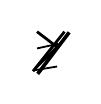
\begin{tikzpicture}[x=0.085mm,y=-0.085mm,baseline=0pt, every node/.style={anchor=base west,inner sep=0pt,outer sep=0pt}]
\path[use as bounding box] (0,0) rectangle (68,72);
\begin{scope}[shift={(-570,-1564)}]
\draw[line width=1.0pt] (584,1570) -- (614,1593) -- (582,1624);
\draw[line width=1.0pt] (625,1570) -- (578,1629);
\draw[line width=.65pt] (584,1595) -- (616,1588);
\draw[line width=.65pt] (578,1628) -- (614,1622);
\draw[line width=1.3pt] (632,1571) -- (585,1633);
\node[overlay] at (576,1617) {\phantom{$\deleted{\unsure{Y|Z|X}}$}};
\end{scope}
\end{tikzpicture}%
}};
% END A022-G13-old-variable
% LABEL T54: owns exactly the visible contents of this node; state=deleted.
\node at (641,1613) {\resizebox{2.635mm}{!}{\rlap{$=$}\phantom{\deleted{$=$}}}};
% BEGIN A022-S14
% Observed locus [716, 1540, 827, 1624]; complete ownership: complete Sigma body, head, hat, raised sign and index; no adjacent relation or word
% Complete candidate/state annotation: \widehat{\Sigma}_{\alpha}^{-}
\draw[line width=.7pt] (726,1582) -- (772,1581);
\draw[line width=.7pt] (723,1588) -- (756,1595) -- (721,1614) -- (773,1610);
\draw[line width=.7pt] (758,1564) -- (782,1550) -- (799,1561);
\node at (799,1587) {\resizebox{1.445mm}{!}{$-$}};
\node at (783,1622) {\resizebox{1.955mm}{!}{$\alpha$}};
\node[overlay] at (716,1624) {\phantom{$\deleted{\widehat{\Sigma}_{\alpha}^{-}}$}};
% END A022-S14
% LABEL T55: owns exactly the visible contents of this node; state=deleted.
\node at (855,1610) {\resizebox{1.615mm}{!}{\rlap{$=$}\phantom{\deleted{$=$}}}};
% BEGIN A022-S15
% Observed locus [894, 1572, 985, 1627]; complete ownership: complete Sigma body, head, raised sign and index; no adjacent relation or word
% Complete candidate/state annotation: \Sigma_{\alpha}^{-}
\draw[line width=.7pt] (903,1582) -- (934,1581);
\draw[line width=.7pt] (901,1589) -- (927,1595) -- (898,1612) -- (939,1612);
\node at (958,1588) {\resizebox{1.445mm}{!}{$-$}};
\node at (943,1625) {\resizebox{1.955mm}{!}{$\alpha$}};
\node[overlay] at (894,1627) {\phantom{$\deleted{\Sigma_{\alpha}^{-}}$}};
% END A022-S15
% LABEL T56: owns exactly the visible contents of this node; state=deleted.
\node at (1007,1612) {\resizebox{11.475mm}{!}{\rlap{$\cup E_\alpha$}\phantom{\deleted{$\cup E_\alpha$}}}};
% LABEL T57: owns exactly the visible contents of this node; state=deleted.
\node at (302,1726) {\resizebox{30.940mm}{!}{\rlap{dans lequel}\phantom{\deleted{dans lequel}}}};
% LABEL T58: owns exactly the visible contents of this node; state=deleted.
\node at (748,1717) {\resizebox{12.155mm}{!}{\rlap{on a}\phantom{\deleted{on a}}}};
% LABEL T59: owns exactly the visible contents of this node; state=deleted.
\node at (950,1718) {\resizebox{47.345mm}{!}{\rlap{deux parties ferm\unsure{è|é|e}es}\phantom{\deleted{deux parties ferm\unsure{è|é|e}es}}}};
% LABEL T60: owns exactly the visible contents of this node; state=deleted.
\node at (304,1841) {\resizebox{23.800mm}{!}{\rlap{disjointes}\phantom{\deleted{disjointes}}}};
% BEGIN A022-G14-cancellation-frame
% Observed locus [256, 768, 1598, 1850]; complete ownership: all long cancellation/frame runs, including the shared upper rule above S11 and the lower continuation around disjointes; adjacent letters/words are owned by their labels/Sigma groups
% Complete candidate/state annotation: enclosing cancellation; exact temporal order and shared-bar authorship are not inferred
\draw[line width=.5pt] (264,836) -- (282,835) .. controls (528,828) and (710,800) .. (1018,788) .. controls (1192,779) and (1331,774) .. (1409,773) -- (1494,773) .. controls (1535,772) and (1564,774) .. (1581,778);
\draw[line width=.5pt] (282,835) .. controls (295,1034) and (305,1230) .. (283,1396) .. controls (279,1481) and (312,1497) .. (312,1597) .. controls (316,1644) and (523,1610) .. (706,1594) .. controls (866,1584) and (1035,1624) .. (1140,1612) .. controls (1243,1608) and (1311,1572) .. (1345,1545);
\draw[line width=.5pt] (516,843) .. controls (588,1000) and (692,1190) .. (786,1273) .. controls (798,1281) and (809,1289) .. (815,1287);
\draw[line width=.5pt] (985,893) .. controls (1050,1046) and (1138,1276) .. (1206,1374) -- (1240,1410);
\draw[line width=.5pt] (1394,847) .. controls (1437,939) and (1487,1069) .. (1501,1154);
\draw[line width=.5pt] (283,1397) .. controls (404,1400) and (535,1390) .. (638,1380) .. controls (627,1357) and (618,1323) .. (634,1305) .. controls (645,1279) and (673,1283) .. (738,1285) .. controls (913,1289) and (1147,1291) .. (1327,1286) .. controls (1336,1284) and (1340,1280) .. (1331,1273);
\draw[line width=.55pt] (815,1329) .. controls (860,1384) and (902,1457) .. (961,1475);
\draw[line width=.55pt] (276,1504) .. controls (447,1495) and (650,1481) .. (908,1476) .. controls (1104,1471) and (1238,1471) .. (1353,1469) .. controls (1439,1467) and (1481,1437) .. (1515,1377) .. controls (1544,1338) and (1565,1328) .. (1597,1319);
\draw[line width=.5pt] (308,1734) .. controls (570,1721) and (826,1714) .. (1050,1710) .. controls (1238,1707) and (1411,1706) .. (1515,1712);
% Root §11: the following two literal B022-G14 paths retain their interruption.
\draw[line width=.3pt,line cap=round] (308,1736) .. controls (302,1762) and (298,1787) .. (296,1804);
\draw[line width=.35pt,line cap=round] (296,1809) .. controls (294,1839) and (330,1848) .. (377,1840) .. controls (467,1832) and (540,1828) .. (590,1823) .. controls (638,1820) and (648,1810) .. (627,1745);
% END A022-G14-cancellation-frame% BEGIN B022-M07; observed full-scan box [1649, 1725, 1665, 1743].
% Ownership: Two separate small points near the right paper edge, beside the lower cancelled/live transition; no adjoining word.
% Role/state: Both shapes are supported; attachment, role, hand and surface origin remain unresolved.
% Complete reading/state candidates: two small points; no punctuation assigned
\node[anchor=base west,inner sep=0pt,outer sep=0pt] at (1649,1743) {\unsure{%
\begin{tikzpicture}[x=0.085mm,y=-0.085mm,baseline=(B),every node/.style={inner sep=0pt,outer sep=0pt,anchor=base west}]
\path[use as bounding box] (0,0) rectangle (16,18);
\coordinate (B) at (0,18);
\begin{scope}[shift={(-1649,-1725)}]
\fill (1658.1,1729.3) .. controls (1659.1,1728.3) and (1661.0,1729.1) .. (1660.8,1730.5) .. controls (1660.5,1732.0) and (1658.2,1732.3) .. (1657.7,1731.0) -- cycle;
\fill (1653.0,1736.2) .. controls (1654.2,1735.5) and (1655.9,1736.2) .. (1655.7,1737.7) .. controls (1655.1,1739.0) and (1652.9,1738.8) .. (1652.8,1737.2) -- cycle;
\end{scope}
\end{tikzpicture}%
}};
% END B022-M07

% LABEL T61: owns exactly the visible contents of this node; state=live.
\node at (718,1792) {\resizebox{68.170mm}{!}{Or dans $X$ on a les deux}};
% LABEL T62: owns exactly the visible contents of this node; state=live.
\node at (306,1926) {\resizebox{17.085mm}{!}{parties}};
% LABEL T63: owns exactly the visible contents of this node; state=live.
\node at (581,1902) {\resizebox{16.235mm}{!}{fermées}};
% LABEL T64: owns exactly the visible contents of this node; state=live.
\node at (841,1894) {\resizebox{23.120mm}{!}{disjointes}};
% BEGIN A022-G15-live-underlines
% Observed locus [630, 1898, 1114, 1930]; complete ownership: the two physical underline runs under fermées and disjointes; both word labels remain outside
\draw[line width=.65pt] (634,1926) .. controls (681,1920) and (718,1917) .. (758,1914);
\draw[line width=.65pt] (873,1908) .. controls (947,1905) and (1028,1903) .. (1107,1902);
% END A022-G15-live-underlines
% BEGIN A022-M03-fermees-upper-tick
% Observed locus [726, 1875, 735, 1888]; complete ownership: short detached upper tick before the clear acute of live fermées; the word and acute remain T63
\node[anchor=base west,inner sep=0pt,outer sep=0pt] at (726,1875) {\unsure{%
\begin{tikzpicture}[x=0.085mm,y=-0.085mm,baseline=0pt, every node/.style={anchor=base west,inner sep=0pt,outer sep=0pt}]
\path[use as bounding box] (0,0) rectangle (9,13);
\begin{scope}[shift={(-726,-1875)}]
\draw[line width=.8pt] (731,1879) -- (729,1885);
\end{scope}
\end{tikzpicture}%
}};
% END A022-M03-fermees-upper-tick
% BEGIN A022-M04-detached-slash
% Observed locus [1213, 1830, 1241, 1857]; complete ownership: one detached down-right slash above-right of disjointes; adjoining words are outside
\node[anchor=base west,inner sep=0pt,outer sep=0pt] at (1213,1830) {\unsure{%
\begin{tikzpicture}[x=0.085mm,y=-0.085mm,baseline=0pt, every node/.style={anchor=base west,inner sep=0pt,outer sep=0pt}]
\path[use as bounding box] (0,0) rectangle (28,27);
\begin{scope}[shift={(-1213,-1830)}]
\draw[line width=.7pt] (1218,1836) -- (1236,1851);
\end{scope}
\end{tikzpicture}%
}};
% END A022-M04-detached-slash
% LABEL T65: owns exactly the visible contents of this node; state=live.
\node at (639,2026) {\resizebox{5.270mm}{!}{$Y=$}};
% BEGIN A022-S16
% Observed locus [716, 1948, 812, 2033]; complete ownership: complete Sigma body, head, hat, raised sign and index; no adjacent relation or word
% Complete candidate/state annotation: \widehat{\Sigma}_{\alpha}^{+}
\draw[line width=.7pt] (729,1978) -- (766,1977);
\draw[line width=.7pt] (729,1978) -- (754,1991) -- (723,2016) -- (777,2018);
\draw[line width=.7pt] (740,1965) -- (778,1953) -- (795,1964);
\node at (786,1980) {\resizebox{1.445mm}{!}{$+$}};
\node at (774,2030) {\resizebox{1.955mm}{!}{$\alpha$}};
% END A022-S16
% LABEL T66: owns exactly the visible contents of this node; state=live.
\node at (832,2046) {\resizebox{1.615mm}{!}{,}};
% LABEL T67: owns exactly the visible contents of this node; state=live.
\node at (906,2003) {\resizebox{7.140mm}{!}{$Z\phantom{=}$}};
% Root import C022-G09: original parent origin (635,2021), original parent node anchor (340,-15).
% Copied declared full base-west anchor (975,2006), inner box xmin=-4, inner origin (979,2006).
\node[anchor=base west,inner sep=0,outer sep=0,font=\small] at (975,2006) {\unsure{\mbox{% BEGIN C022-G09
% observed full-scan bbox (975, 1991, 998, 2010); origin/baseline (979, 2006).
% Local x=X-979, y=Y-2006; x=0.085mm, y=-0.085mm.
% Owns the small paired/returning relation after Z, primary equals with unresolved right-end join; no Z letter or union.
\begin{tikzpicture}[baseline={(0,0)},x=0.085mm,y=-0.085mm,line cap=round,line join=round]
\path[use as bounding box] (-4,-15) rectangle (19,4);
\draw[line width=.4pt] (0,-8) .. controls (7,-12) and (15,-10) .. (13,-5) .. controls (9,-2) and (4,-1) .. (0,-2);
\node[anchor=base west,inner sep=0,outer sep=0,font=\small,overlay] at (0,0) {$\phantom{\unsure{=}}$};
\end{tikzpicture}
% END C022-G09
}}};
% BEGIN A022-G16-final-union
% Observed locus [1013, 1953, 1207, 2086]; complete ownership: final indexed union body and its beta-in-K-setminus-alpha limit; adjoining Z and Sigma S17 remain separate
\draw[line width=.65pt] (1043,1963) .. controls (1045,1984) and (1045,2018) .. (1063,2019) .. controls (1085,2020) and (1110,1994) .. (1107,1963);
\node at (1018,2078) {\resizebox{16.150mm}{!}{$\beta\in K\setminus\{\alpha\}$}};
% END A022-G16-final-union
% BEGIN A022-S17
% Observed locus [1194, 1928, 1298, 2040]; complete ownership: complete Sigma body, head, hat, raised sign and index; no adjacent relation or word
% Complete candidate/state annotation: \widehat{\Sigma}_{\beta}^{+}
\draw[line width=.7pt] (1203,1964) -- (1246,1963);
\draw[line width=.7pt] (1203,1972) -- (1234,1985) -- (1199,2000) -- (1253,2000);
\draw[line width=.7pt] (1239,1947) -- (1258,1933) -- (1278,1944);
\node at (1279,1971) {\resizebox{1.445mm}{!}{$+$}};
\node at (1259,2037) {\resizebox{2.295mm}{!}{$\beta$}};
% END A022-S17
% BEGIN B022-M04; observed full-scan box [1205, 1973, 1218, 1986].
% Ownership: The small inner triangular point of the S17 complete glyph cluster; no Sigma or beta is duplicated.
% Role/state: Shape high confidence; attachment, role, hand and surface origin unresolved.
% Complete reading/state candidates: small point within the Sigma arms; no operation assigned
\node[anchor=base west,inner sep=0pt,outer sep=0pt] at (1205,1986) {\unsure{%
\begin{tikzpicture}[x=0.085mm,y=-0.085mm,baseline=(B),every node/.style={inner sep=0pt,outer sep=0pt,anchor=base west}]
\path[use as bounding box] (0,0) rectangle (13,13);
\coordinate (B) at (0,13);
\begin{scope}[shift={(-1205,-1973)}]
\fill (1210,1977) -- (1214,1980) -- (1208,1981) -- cycle;
\end{scope}
\end{tikzpicture}%
}};
% END B022-M04

% BEGIN A022-M06-below-beta-point
% Observed locus [1282, 2042, 1292, 2054]; complete ownership: one tiny point below-right of S17 beta; the beta remains in S17
\node[anchor=base west,inner sep=0pt,outer sep=0pt] at (1282,2042) {\unsure{%
\begin{tikzpicture}[x=0.085mm,y=-0.085mm,baseline=0pt, every node/.style={anchor=base west,inner sep=0pt,outer sep=0pt}]
\path[use as bounding box] (0,0) rectangle (10,12);
\begin{scope}[shift={(-1282,-2042)}]
\fill (1287,2048) circle[radius=.7];
\end{scope}
\end{tikzpicture}%
}};
% END A022-M06-below-beta-point
\end{tikzpicture}}

et on doit prouver
\[
\overline{(X\setminus(Y\cup Z))}\cap Y=\overline{(X\setminus Y)}\cap Y
\]
ce qui est immédiat
% archive sheet number: 21
